\documentclass[10pt,letterpaper]{article}
\usepackage[utf8]{inputenc}
\usepackage{amsmath}
\usepackage{amsfonts}
\usepackage{amssymb}
\usepackage{graphicx}
\author{Brock Ellefson}
\title{CSCI 432}
\begin{document}
\maketitle
\section{Prove that a tree with n vertices has n-1 edges}
For each node, there is always an edge. The only exception is the root node, which gives the n-1 edges.
	\begin{figure}[h]
	    \caption{As you can see here. Every nodes have an edge except for the root node, giving us n-1 edges.}
		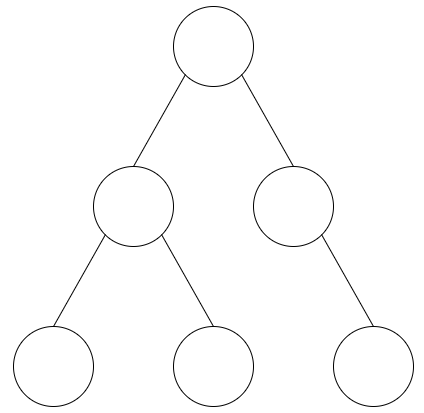
\includegraphics[scale = .25]{CSCI432HW1TreeExample.png}
  		\label{fig:PCP}
	\end{figure}
\section{Choose three algorithms from EPI and state in your own words what the algorithm}	
	\subsection*{isSymmetric}
		isSymmetric is an algorithm that checks to see if a binary tree is symmetric. It does this by checking subtrees within the original tree and using short-circuit evaluation if any subtree test fails.
	\subsection*{binarySearch} 
		Binary Search is an algorithm that checks to see if a value is within a sorted array. It takes the first, last, and middle element in the array, evaluates whether the middle element is bigger or smaller than the desired element. Then that mid will be reassigned as the new high or low and cute this sub array in half and repeats this process until the element is either found or if the mid exasperated all of the elements in the array.
	\subsection*{quickSort}
		Quicksort is a sorting algorithm that implements a divide and conquer strategy by breaking down an array into little pieces and sorting the small pieces.
		



\end{document}